

%% The command below calls the preprint style
%% which will produce a one-column, single-spaced document.
%% Examples of commands for other substyles follow. Use
%% whichever is most appropriate for your purposes.
%%
%%\documentclass[12pt,preprint]{aastex}

%% manuscript produces a one-column, double-spaced document:

%% \documentclass[manuscript]{aastex}

%% preprint2 produces a double-column, single-spaced document:

\documentclass[preprint2]{aastex}

%% Sometimes a paper's abstract is too long to fit on the
%% title page in preprint2 mode. When that is the case,
%% use the longabstract style option.

%% \documentclass[preprint2,longabstract]{aastex}

%% If you want to create your own macros, you can do so
%% using \newcommand. Your macros should appear before
%% the \begin{document} command.
%%
%% If you are submitting to a journal that translates manuscripts
%% into SGML, you need to follow certain guidelines when preparing
%% your macros. See the AASTeX v5.x Author Guide
%% for information.

\newcommand{\vdag}{(v)^\dagger}
\newcommand{\myemail}{dschaffner@gmail.com}

%% You can insert a short comment on the title page using the command below.

%%\slugcomment{Not to appear in Nonlearned J., 45.}

%% If you wish, you may supply running head information, although
%% this information may be modified by the editorial offices.
%% The left head contains a list of authors,
%% usually a maximum of three (otherwise use et al.).  The right
%% head is a modified title of up to roughly 44 characters.
%% Running heads will not print in the manuscript style.

%%\shorttitle{Collapsed Cores in Globular Clusters}
%%\shortauthors{Djorgovski et al.}

%% This is the end of the preamble.  Indicate the beginning of the
%% paper itself with \begin{document}.

%AIP Reprint Class%%%%%%%%%%%%%%%%%%%%%%%%%%%%%%%%%%%%%%%%%%%%%%%%%%%%%%%%%%%%%%%%%%%%%%%%%%%%%
%\documentclass[aip,prl,amsmath,amssymb,reprint,superscriptaddress]{revtex4-1} %preprint version
%\usepackage{graphicx}% Include figure files
%\usepackage{dcolumn}% Align table columns on decimal point
%\usepackage{bm}% bold math
%\usepackage{epstopdf}

%    \renewcommand{\topfraction}{0.9}    % max fraction of floats at top
%    \renewcommand{\bottomfraction}{0.8}    % max fraction of floats at bottom
%    \setcounter{topnumber}{2}
%    \setcounter{bottomnumber}{2}
%    \setcounter{totalnumber}{4}     % 2 may work better
%    \setcounter{dbltopnumber}{2}    % for 2-column pages
%    \renewcommand{\dbltopfraction}{0.9}    % fit big float above 2-col. text
%    \renewcommand{\textfraction}{0.07}    % allow minimal text w. figs
%    \renewcommand{\floatpagefraction}{0.7}    % require fuller float pages
%    \renewcommand{\dblfloatpagefraction}{0.7}    % require fuller float pages
%    \setlength{\abovecaptionskip}{5pt}
%    \setlength{\belowcaptionskip}{5pt}
%    \setlength{\parskip}{0pt}
%    \setlength{\textfloatsep}{5pt} 

%%%%%%%%%%%%%%%%%%%%%%%%%%%%%%%%%%%%%%%%%%%%%%%%%%%%%%%%%%%%%%%%%%%%%%%%%%%%%%%%%%%%%%%%%%%%%%%%%%

\begin{document}
\title{Multifractal and monofractal scaling in a laboratory MHD turbulence experiment}

\author{D.A. Schaffner and M.R. Brown}
\affil{Swarthmore College, Swarthmore, PA, USA}

\date{\today}
\begin{abstract}
Both multifractal and monofractal scaling of structure function exponents are observed in the turbulent magnetic fluctuations of the Swarthmore Spheromak Experiment (SSX) plasma. Structure function and probability distribution function (PDF) analysis exhibits mulitfractal scaling exponents in low frequency, inertial range fluctuations of the turbulence but monofractal scaling in higher frequency, dissipation range fluctuations. The transition from multifractal to monofractal scaling occurs rapidly suggesting a dissipation mechanism that is insensitive to turbulent structure scale size. Structure functions and PDFs are presented for both temporal and spatial measurements. Variations in the magnetic helicity in the plasma are also shown to modify multifractal scaling characteristics of the inertial range, but do not affect the monofractal scaling of the dissipation range.
\end{abstract}

\keywords{plasmas,MHD,turbulence,methods: laboratory}

\section{Introduction}

This paper presents the results of a thorough intermittency analysis of the fluctuating magnetic fields in the Swarthmore Spheromak Experiment (SSX) plasma through the use of structure functions and probability distribution functions (PDFs) of increments of both temporal and spatial measurements. The primary observation from this analysis is that temporal regions of the magnetic fluctuation data that are shown to be consistent with dissipation range turbulence~\citep{schaffner2014c} exhibit structure function scaling that indicates self-similar structure, whereas temporal regions consistent with inertial range turbulence do not exhibit this self-similarity. These results are discussed in the context of multifractal versus monofractal structure function scaling behavior of turbulence~\citep{paladin1987,frisch1995,marsch1997}, where a lack of self-similarity can be attributed to multifractal behavior of the system. Similar distinctions between inertial range and dissipation range scaling are made in recent solar wind observations~\citep{kiyani2013} suggesting that physical mechanisms underlying the scaling in each regime may be universal between solar wind and laboratory based MHD turbulence. Furthermore, the relatively fast transition from multifractal to monofractal scaling suggests a dissipation mechanism which may have an absolute scale, such as the generation of current sheets at the ion inertial scale length~\citep{kiyani2009,kiyani2010}, and not one that is relative to the scale size of structures in the inertial range such as that observed in conventional fluid turbulence~\citep{chevillard2005}.

Trends in scaling with magnetic helicity injection are also explored. Previous work~\citep{schaffner2014b} demonstrated that increased injected helicity in the SSX plasma system resulted in an increased intermittency of the raw $dB(t)/dt$ signal. Results reported here show that $B(t)$ formed from time integration of the raw $dB(t)/dt$ signal exhibit this same trend. The scaling behavior of the structure functions differ with helicity depending on whether they are constructed from data in the dissipation versus the inertial range. Inertial range scaling appears to vary more widely with helicity than the dissipation range. This indicates variation of helicity injection has an affect only on intermittent structures generated in the inertial range, or on the physical mechanism which does the generating. Conversely, the mechanism that governs intermittency in the dissipation range is not strongly affected by the overall helicity content of the plasma.

Structure function analysis has typically been utilized to extend spectral or correlation analysis of turbulent fluctuations to higher-order statistics, particularly in scenarios where Gaussian and self-similar properties appear to break down. Examined first in hydrodynamics~\citep{anselmet1984,frisch1995}, the use of the technique has been expanded to magnetohydrodynamic (MHD) fluids including the solar wind velocity fluctuations~\citep{burlaga1991}, solar wind magnetic fluctuations~\citep{burlaga1992,tu1995} and magnetospheric plasmas~\citep{consolini1996,hnat2003}. The work has led to the development of models which attempt to reconcile the observation of intermittency and non-self-similar statistics in turbulence fluctuations with the 1941 Kolmogorov turbulence model which implies a self-similar fluctuation structure, and which can be described in terms of a monofractal scaling exponent~\citep{kolmogorov1941,frisch1995}. Such multifractal models relax global scale invariance to a local scale invariance. Physically, these models describe modifications of how energy is distributed to smaller scales from larger scales either through differences in the space-filling nature of the turbulence, such as the random $\beta$-model~\citep{benzi1984} or through variations in the energy transfer rate from larger to smaller scales such as the log-normal model~\citep{kolmogorov1962}, the $p$-model~\citep{meneveau1987} and the She-Leveque model~\citep{she1994,dubrulle1994}. Multifractal scaling models can make predictions for dissipation scaling, in particular addressing a reduction in scaling exponents by viscosity~\citep{frisch1991,chevillard2005}. Since these models were developed with isotropic and homogeneous turbulence of conventional neutral fluids, extending intermittency models to MHD turbulence has added complications. MHD turbulence is inherently anisotropic---due to the symmetry breaking caused by embedded magnetic fields---in addition to having fluctuations, energy transfer and dissipation channels for both magnetic and velocity fields. While hydrodynamic intermittency models have been directly applied to MHD turbulence~\citep{burlaga1991,pagel2002}, modified models pertaining explicitly to MHD have also been developed~\citep{carbone1993,biskamp1994,muller2000,biskamp2000,boldyrev2002,cho2003}. Structure function analysis can be of particular use for extracting signatures of dissipation in MHD turbulence~\citep{cho2003,alexandrova2008,kiyani2009,kiyani2013}.

\section{Experiment}\label{sec:experiment}

Magnetohydrodynamic turbulent fluctuations are produced inside the compact wind tunnel configuration of the Swarthmore Spheromak Experiment (SSX) using a plasma gun source inside a flux-conserving copper boundary. A turbulent cascade is generated by the injection of large scale (size of the column radius) magnetic structures by the gun which evolve and relax under the constraint of constant magnetic helicity inside the flux-conserving column, transferring energy to smaller scales~\citep{schaffner2014c}. The copper cylinder is 15.5cm in diameter and 86cm long and situated inside a highly-evacuated chamber ($\approx 1 \times 10^{-8}$ Torr). The details of the gun source and production of magnetic fluctuations have been previously reported~\citep{schaffner2014c,brown14,brown15a}. The gun produces a 120$\mu s$ discharge of plasma; though the plasma is pulsed, there is a window of time in which the energy input from the gun roughly balances the energy loss in the system, generating a period of stationarity of fluctuations~\citep{schaffner2014a,brown14,brown15a}. This time range, from 40 to 60$\mu s$ after initiation of the discharge, is extracted from each shot to form an ensemble for analysis. The diagnostic analyzed in this paper is of magnetic fluctuations using an array of sixteen magnetic pickup channels. Each channel consists of a single-loop of magnetic wire, 3mm in diameter. Three loops are oriented in each cylindrical coordinate direction ($B_{r},B_{\theta},B_{z}$) and each triplet is separated by 0.46cm spanning from about 1cm off the cylindrical axis to the edge of the cylinder boundary. The injected helicity of the plasma is scanned from $0$ to $7\times 10^{-5}~Wb^{2}$ which corresponds to a scan of the amount of flux provided to the gun core--from $0$ to $1.5~mWb$~\citep{schaffner2014b}.

\section{Analysis Techniques}\label{sec:analysis}

The structure functions and PDFs are constructed by taking differences or increments at varying time or spatial separations. In this analysis, the increments of magnetic measurements are constructed in three ways; first, the increments of each orthogonal magnetic component ($\Delta B_r$,$\Delta B_{\theta}$,and $\Delta B_z$) are examined separately. Then, vector magnitude is created from the vector sum of the three components at each time step and differences between the magnitudes ($\Delta |B|$) at each time step are used for the analysis. Lastly, the magnitude of the vector difference between time points is used as the increment ($|\Delta B|$). The increments can be in terms of a spatial division or a temporal division. In the context of this experiment, the spatial increments are in units of separation distance between probe locations ($\Delta r_{min} = 0.46cm$), while the temporal increments are in units of sampling cadence ($\Delta \tau_{min} = 15.4ns$) which corresponds to the sampling frequency of 65MHz. Increments are then increased in multiples of these minimum values. Maximum separation values are limited by physical distance or data acquisition time span, as well as the ability to generate enough statistics for a valid calculation, though the main focus of results here will be on scales much smaller than the available time span to avoid issues of non-stationarity.

For a given increment, $\Delta x$, the PDF of increments is constructed by computing and histogramming a list of $\Delta B$'s,
\begin{equation}
\Delta B = |B(x+\Delta x)-B(x)|
\label{eq:increment}
\end{equation}
which can then be normalized to the standard deviation and the total number of increments available in the dataset for each given $\Delta x$.

A  PDF can describe the nature of the data in terms of its relative distribution with respect to a Gaussian distribution. Large excursions of values in the tail values of the distribution are then indicative of intermittent behavior in the time series signal---i.e. large jumps in values outside of the standard deviation of the mean. Physically, these excursions can be identified with mechanisms in the plasma such as current sheets or shocks.

Further insight into the physical nature of the plasma can be gained by comparing these PDFs over a range of scales. This can be accomplished qualitatively by examining how the PDFs themselves change, but can also be quantitatively accomplished by calculating moments of these distributions: these are the structure functions. The structure function can be constructed for a given $\Delta x$ by computing the average of the increments raised to some order, $p$, as in,
\begin{equation}
S^{p}(\Delta x) = \langle|B(x_{j}+\Delta x)-B(x_{j})|^{p}\rangle
\label{eq:structfunc}
\end{equation}
again where $j$ indicates the available increments to be summed over. 

Analysis of structure functions can illuminate characteristics of the fluctuations particularly when modeled as a power-law function,
\begin{equation}
S^{p}(\Delta x) = (\Delta x)^{\zeta}.
\label{eq:power-law}
\end{equation}
When plotted logarithmically, $\zeta$ is the slope of the structure function; this slope can indicate the relative level of intermittency compared between two signals. That is, the steeper the slope, the more intermittent (i.e. the larger the ``fat tails'') is the signal. A flat line is the extreme case and indicates a lack of intermittency in the signal. As one would expect, the structure function of a timeseries generated from a normal distribution has a flat structure function. Changes in slope with scale indicates a change in intermittency as a function of scale. It should be noted, however, that this trend is not a perfect predictor of the presence of intermittency. For example, it can be shown that a time-series of fractional Brownian motion (fBm) can be constructed with the same structure function slope~\citep{hnat2003}, but fBm produces a Gaussian probability distribution of increments. However, when intermittency is known to be present based on the PDF of increments (as is true for this SSX dataset) then the relationship between slope and degree of intermittency generally holds true.

If $\zeta$ scales as a linear function of order $p$ (i.e. $\zeta(p) = Hp$), the system exhibits self-similarity at different scales. In this context, the self-similarity is a qualitative measure of how alike fluctuations appear at different scales. For example, a fractal from chaos theory is a construct that exhibits self-similarity. In other words, a self-similar system can be described in terms of a single fractal scaling or monofractal scaling description. The constant coefficient, $H$, is called the Hurst exponent; it can be shown that distributions that exhibit this self-similarity can be rescaled using the Hurst exponent as,
\begin{equation}
PDF(\Delta B,\Delta x^{-H}) = (\Delta x)^HPDF(\Delta B,\Delta x)
\label{eq:scaling}
\end{equation}
A non-linear $\zeta(p)$, however, indicates non-self-similar behavior, exhibiting multiple fractal scalings simultaneously (i.e. multifractal behavior). These distinctions again can be used to elucidate possible physical mechanisms at play in the plasma. 

In particular, it has been shown that differences in self-similarity exist between inertial range and dissipation range data in the solar wind~\citep{kiyani2009,kiyani2013}. The slope of the structure functions of the solar wind inertial range were not linear as a function of order, indicating that these inertial range turbulent fluctuations do not exhibit self-similarity of turbulent structure, and can be considered multifractal. On the other hand, the same analysis for dissipation range structure functions exhibited linear scaling---apparently, the physical mechanism behind the dissipation in the solar wind has a self-similar, scale-invariant nature---that is, monofractal behavior.

\section{Temporal and Spatial PDFs of Increments}\label{sec:pdfs}

\begin{figure*}
\epsscale{1.0}
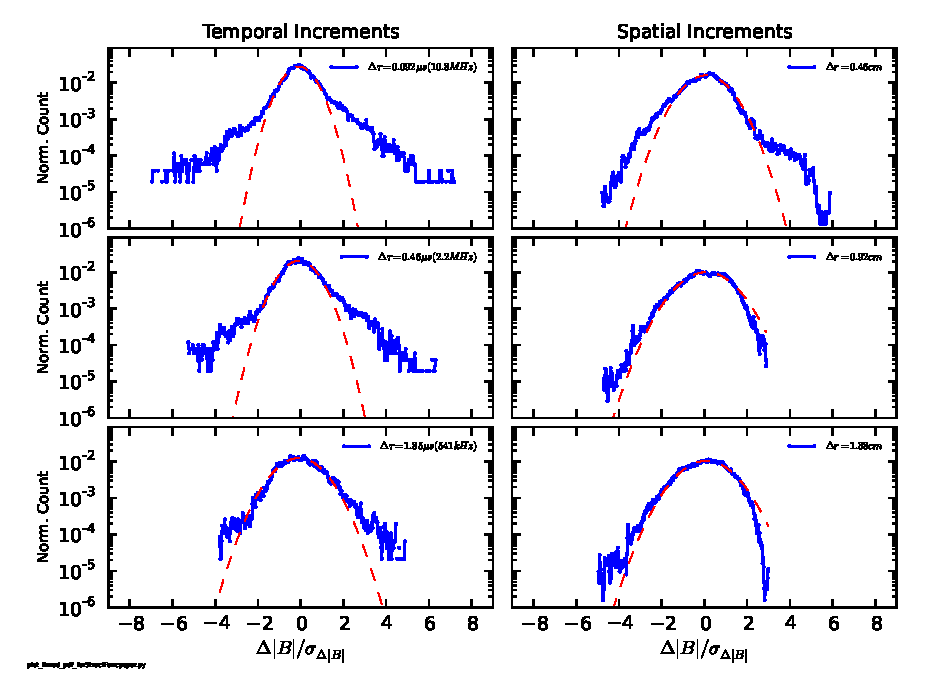
\includegraphics{fig1.eps}
\caption{\label{fig:pdfs}Probability Distribution Functions (PDFs) of increments for (a-c) temporal and (d-f) spatial measurements of $\Delta |B|$. The temporal increments are (a)$0.092\mu s$, (b)$0.46\mu s$, and (c)$1.85\mu s$ while the spatial increments are (d)$0.46$cm, (e)$0.92$cm, and (f)$1.38$cm. Both temporal and spatial PDFs exhibit non-Gaussian tails indicating intermittency (Gaussian distributions are indicated with dashed red lines), but that the level of intermittency decreases with increasing increment. Spatial PDFs appear to be slightly more asymmetric which may be a result of boundary effects or low resolution compared with temporal measurements.}
\end{figure*}

Representative PDFs of both temporal and spatial magnetic field magnitude ($\Delta |B|$) increments are shown in Figure~\ref{fig:pdfs} with temporal PDFs on the left and spatial PDFs on the right. Each PDFs is scaled to its own standard deviation and total count so that they can be cross compared. The increments chosen for the temporal PDFs are $0.092\mu s$, $0.46\mu s$, and $1.85\mu s$ which correspond to frequencies of $10.8MHz$, $2.2MHz$, and $541kHz$ respectively. These three times also approximately correspond to three different regimes of the frequency spectra, called for lack of more accurate description the dissipation, transition and inertial region. All three PDFs exhibit intermittent behavior as indicated by the wings or ``fat tails'' for large fluctuation values which reflect larger counts compared to a true Gaussian distribution which is indicated by the dashed red curves. Note, though, that the qualitative ``level'' of intermittency decreases with increasing temporal increment, consistent with previous intermittency analyzes on SSX~\citep{schaffner2014a,schaffner2014b}, as well as solar wind results~\citep{bruno2013}.

The increments chosen for the spatial PDFs are $0.46cm$, $0.92cm$, and $1.38cm$, which corresponds to the minimum, double the minimum, and triple the minimum separation possible given the probe array in the SSX. Unlike the temporal data, the spatial data is not believed to probe as far into dissipation range scales (for reference, an ion inertial length of 0.6cm  and an ion gyroradius of 0.1cm is calculated for this plasma). Thus the spatial data is likely representative of inertial range turbulence and at most transition range. The resulting PDFs support this notion as they tend to have a more Gaussian-like distribution for small fluctuations and only slightly elevated tails. There does appear to be a trend toward increasing Gaussian-ness with increasing increment similar to the temporal data. The curves do not appear as smooth as the temporal data though, as the histograms have larger breaks---in particular, the $0.46cm$ increment PDF. This potentially reflects both a lower amount of increment statistics available for the spatial measurement as well as effects due to spatial variation of the plasma. Asymmetry of the spatial PDFs can also be seen; however, this is likely due to influences of the boundary of which the temporal data is much less susceptible. Finer resolution of the spatial measurements would also likely improve the symmetry of the PDFs in addition to allowing observation of the dissipation scale; such improved measurements are currently being attempted.

As discussed before, the use of PDFs of increments can clearly demonstrate the lack or presence of intermittent behavior in a signal, however in a primarily qualitative way. Structure function analysis is needed to unearth the fractal scaling nature of the turbulence.

\section{Structure Functions and Scaling with Order}\label{sec:structs}

To produce a more quantitative metric from the PDFs of increments, one can calculate moments of the histogram to any order $p$, and for each time or spatial delay $\Delta x$. This is equivalent to calculating the structure function in Equation~\ref{eq:structfunc} for the magnetic field increments. Integer values of $p$ correspond to the moments of the PDF ($p=2$ is the second moment, $p=3$ is the third moment, etc.) though given the form of Equation~\ref{eq:structfunc}, $p$ is not restricted to integer values in the structure function formalization.

\begin{figure*}
\epsscale{1.0}
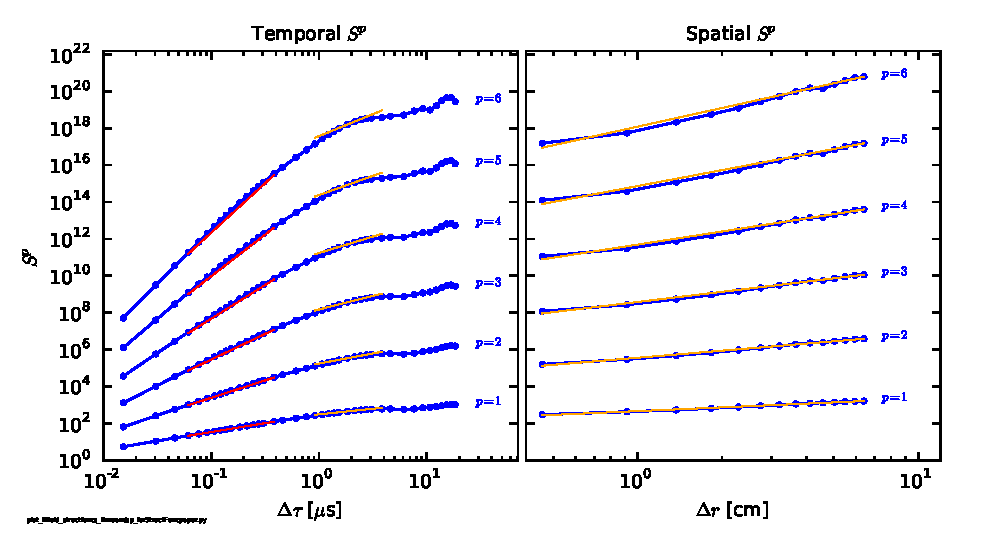
\includegraphics{fig2.eps}
\caption{\label{fig:structfuncs} Structure functions of temporal (left) and spatial (right) measurements for integer orders $p=1$ to $p=6$. Fits to regions of the temporal structure functions are made to compute scaling exponents, $\zeta$; separate regions are selected based on the breakdown of the frequency spectrum shown in Schaffner 2014c which occurs at approximatly 1MHz or 1$\mu s$. Spatial measurements likely span only the inertial range and thus only one region is fit. }
\end{figure*}

\begin{figure}
\epsscale{1.0}
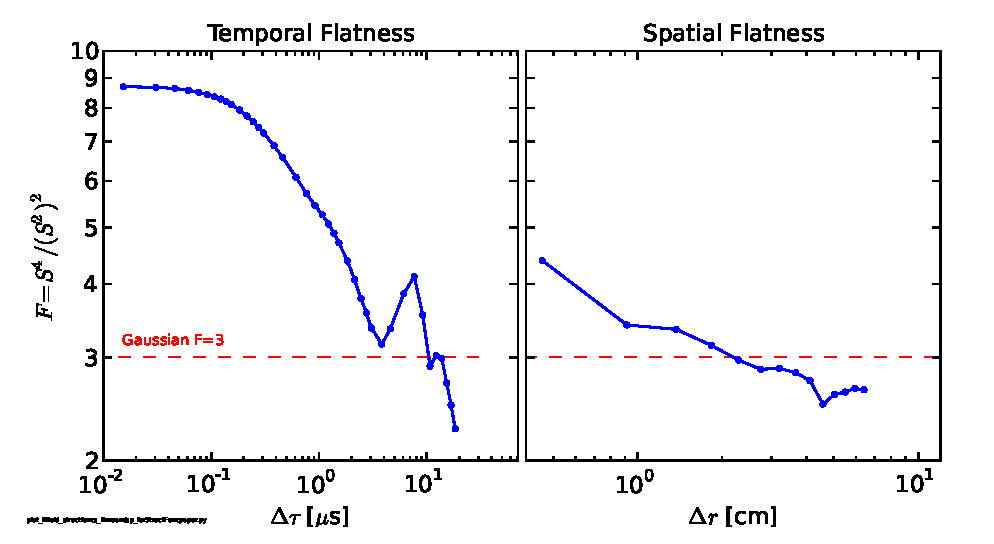
\includegraphics[width={\columnwidth}]{fig3.eps}
\caption{\label{fig:flatness} Normalized fourth order structure functions (a.k.a flatness or kurtosis) for temporal (left) and spatial (right) measurements. The flatness of a Gaussian signal is indicated by the dashed line at F=3. Both figures show increasing flatness with decreasing scale indicating a rise in intermittency.}
\end{figure}

Figure~\ref{fig:structfuncs} shows the structure functions, $S^{p}(\Delta x)$, for temporal ($\Delta x = \Delta \tau$) data on the left and spatial ($\Delta x = \Delta r$) data on the right. The integer structure functions from $p=1$ to $p=6$ are shown. The structure functions vary as a function of $\tau$ or $r$ which confirms the presence of intermittency in the signal. For the temporal results, it is clear that this variation changes as a function of time scale, with steeper slopes at small values of $\tau$ transitioning to shallower slopes at large values of $\tau$. This indicates that the relative degree of intermittency of the signal increases when analyzed at smaller scales. The scale where the slope changes is consistent with the transition from the inertial to the dissipation range of the cascade as determined by the change in spectral index of the frequency spectrum for this plasma~\citep{schaffner2014c}. This difference between inertial and dissipation range intermittency suggests that the physical mechanism underlying the dissipation dynamics has a stronger intermittent nature. Explanations for this behavior in the solar wind typically focus on the presence of current sheets in the magnetic turbulence~\citep{osman2014}. The observation of this difference between dissipation and inertial range fluctuations in this laboratory plasma also suggests the existence of current sheets~\citep{schaffner2014b}. 

The spatial structure functions do not show a change in slope with scale; the magnitude of the slope, and thus the degree of intermittency, is consistent with the temporal structure functions in the inertial range. Since the spatial measurements can only probe inertial range scales in the plasma, this result supports the distinction between dissipation and inertial range intermittency seen in the temporal data.

It can also be instructive to normalize the structure functions and in particular highlight the ``level'' of non-Gaussianness of a distribution. A normalized structure function can be constructed as,
\begin{equation}
S_{norm}^{p}(\Delta x) = \frac{S^{p}(\Delta x)}{(S^2(\Delta x))^{(p/2)}}
\label{eq:normstructfunc}
\end{equation}
where $p$ is the order of the moment. Using this normalized structure function, a Gaussian timeseries would have a constant value. For example, for $p=4$, this quantity becomes the flatness or kurtosis. Figure~\ref{fig:flatness} shows the flatness for both temporal and spatial data. A Gaussian timeseries would have a constant value of 3. Both Figure~\ref{fig:flatness}(a) and (b) show an excursion from a Gaussian distribution at smaller increments, though it is clearly more pronounced for the temporal data.

The self-similarity or fractal behavior of the turbulence, can be extracted from the structure function analysis by examining the slope of the structure functions as a function of order. The red lines in Figure~\ref{fig:structfuncs} are fits to the structure functions. In the temporal data, fits are applied to two separate regions that correspond to the dissipation and inertial regions based on spectral frequency analysis, while the spatial data has only one fit for the entire region. A fit is made in each of these regions for each structure function using order $p$ which ranges between $0.1$ and $10$ in steps of $0.1$. The results of this scan are displayed in Figure~\ref{fig:slopevsmom} for both time and space. The five separate magnetic field measurements are shown now, with inertial range fits indicated by solid lines and dissipation range fits indicated with dashed lines. In this construction, a timeseries that exhibits self-similarity or monofracticality would produce a line with a constant slope. As the increments are raised to increasingly higher powers, the value of the structure function should also increase power-law like. If the signal is self-similar, an increment between two points in the time series at one scale should have on average the same relative increment between two points at a different scale. In other words, a big fluctuation compared to a small fluctuation at one scale should appear to have the same relative ratio at a different scale. Thus, the structure function should change at a constant rate based on this ratio. If the signal is not self-similar, then the ratio is not constant and differences are increasingly accentuated by the raised exponent resulting in a non-linear scaling.

Since the original Kolmogorov turbulence theory~\citep{kolmogorov1941} assumes a self-similar scaling, it predicts that the structure function slope should be one-third the order, or $\zeta = p/3$. The dashed purple line indicates this prediction in Figure~\ref{fig:slopevsmom}. The inertial range curves for all five temporal magnetic measurements in Figure~\ref{fig:slopevsmom}(a) sit relatively near the Kolmogorov theory line but none of the lines exhibit linear behavior. This indicates that the inertial range fluctuations are multifractal, and not self-similar. The spatial curves in Figure~\ref{fig:slopevsmom}(b) support this observation as they are also non-linear, though less pronounced than for the temporal data.

The dissipation range curves, in contrast, are clearly more linear. This indicates that the dissipation range fluctuations are monofractal while also having a higher level of intermittency than inertial range fluctuations. The Hurst exponents for the dissipation range are consistently about 1 for the various measured B values, steeper than the K41 prediction of H=1/3.

\begin{figure}
\epsscale{1.0}
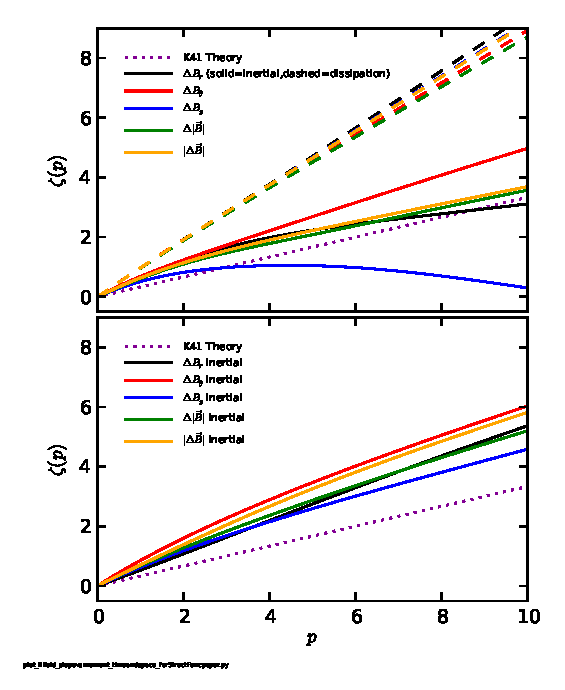
\includegraphics[width={\columnwidth}]{fig4.eps}
\caption{\label{fig:slopevsmom} Scaling exponent, $\zeta$, as a function of structure function order, $p$ for temporal (upper) and spatial (lower) measurements. Inertial range scaling is indicated by the bold lines, while dissipation range scaling is indicated by dashed lines. Temporal scaling shows a clear distinction between multifractal (non-linear $\zeta$ vs $p$) in the inertial range and monofractal (linear $\zeta$ vs $p$) in the dissipation range. The different color curves indicate the type of magnetic structure function used (i.e. B-component, B-vector magnitude, etc.) }
\end{figure}

\section{Helicity Scaling}

The structure function analysis is also used to examine the effect of varying the amount of magnetic helicity in the plasma on the intermittency and self-similarity of the magnetic fluctuations. Previous work has shown that the degree of intermittency in fluctuations of $\dot{B}=dB/dt$ (not $B$), as determined by a calculation of the flatness, increases on average with an increasing amount of injected magnetic helicity~\citep{schaffner2014b}. This work revisits that result by examining the trend in $B$ using unnormalized structure functions and the resulting relationship between structure function slope and $p$. 

\begin{figure}
\epsscale{1.0}
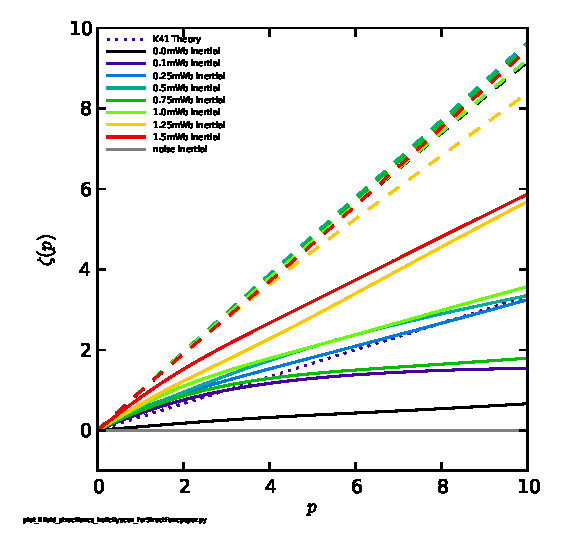
\includegraphics[width={\columnwidth}]{fig5.eps}
\caption{\label{fig:helscan} Scaling exponent versus order for different values of magnetic helicity (as set by the amount of initial flux in the plasma gun~\citep{schaffner2014b}). Inertial range intermittency increases with helicity as shown by increasingly steeper curves in the inertial range. Dissipation range scaling appears to be unaffected by the change in helicity. }
\end{figure}

Figure~\ref{fig:helscan} shows the slope versus order for eight different helicity states for inertial range fluctuations (solid lines) and dissipation range fluctuations (dashed lines). Recalling that the steepness of the slope is indicative of relative degree of intermittency, the order of the inertial range curves for each helicity indicates increasing intermittency with increasing helicity, again consistent with the findings for an analysis of $\dot{B}$ timeseries~\citep{schaffner2014b}. However, the structure function analysis here further shows that with the exception of the zero helicity state, the inertial range turbulence for any helicity is not self-similar. The dissipation range lines, however, show that the dissipation range intermittency is self-similar regardless of the amount of injected magnetic helicity in the plasma.

\section{Discussion}

The observation of both multifractal and monofractal scaling of magnetic fluctuation structure functions in SSX has implications for both the dissipative nature of the turbulence and for the universality of MHD turbulence. Like that observed in Kiyani 2013, the transition between multifractal scaling of the inertial range and monofractal scaling of the dissipation range is rapid. This suggests that the dissipation mechanism is independent of the scale of the turbulence structures---in other words, the dissipation scale is absolute rather than relative. This is in contrast to the predictions and observations made for hydrodynamic turbulence where viscosity is the known dissipation mechanism. In those cases, each scaling exponent has a corresponding dissipation scale due to the viscosity. As smaller and smaller scales are approached, the viscosity ``shuts-off'' the scaling exponents gradually producing a scaling transition region from multifractal inertial to monofractal dissipation ranges~\citep{benzi1984,frisch1991}. If the dissipation mechanism has an absolute scale, independent of each scaling exponent, than a rapid transition would be observed as this absolute scale is passed. Kiyani 2010 discusses this possibility that a dissipation scale associated with the ion inertial length may be at play. However, it is often difficult to distinguish the ion gyroscale ($\rho_i$) effects versus ion inertial scale ($\delta_i$) effects in super-Alfvenic solar wind since $\beta \approx 1$. This laboratory turbulence, however, has a more resolved separation between $\rho_i$ and $\delta_i$~\citep{schaffner2014c}, and the results presented here show the multifractal to monofractal scaling transition occurring at around $\delta_i$ rather than $\rho_i$. Though evidence for the existence of current sheets has been demonstrated in previous SSX experiments on reconnection using stable spheromaks~\citep{brown2012}, more concrete evidence for the presence of current sheets in this more turbulent SSX plasma is still being sought; however, there is preliminary evidence from the helicity scan work~\citep{schaffner2014b} that these current sheets may indeed be present. These current sheets, then, could play the role of an absolute dissipation scale. It should be noted, however, that an alternative solar wind intermittency analysis~\citep{alexandrova2008} does not exhibit a transition in scaling from inertial to dissipation range and the authors of this work suggest the existence of a compressible inertial range cascade rather than a dissipation range.

Another interesting comparison between the results in Kiyani 2013 and those presented here is the difference in collisionality. The solar wind is a collisionless plasma with mean free path lengths on the order of an astronomical unit (AU). The SSX plasma, while still fully ionized, is a collisional plasma with ion mean free path lengths on the order of 0.1cm, a bit less than one order of magnitude smaller than the ion inertial length~\citep{schaffner2014c}. While in MHD turbulence theory, resistivity can be thought to play a role for magnetic turbulence as viscosity would for velocity turbulence, the resistivity does not appear to have the same affect for dissipation given the comparison in scaling between the collisionless solar wind and the collisional laboratory plasma. This result begs the question of what role ion viscosity might have in the turbulent dissipation process as well as indicate possible universality of MHD turbulence regardless of collisionality.

\section{Conclusions}\label{sec:conclusions}

This paper has presented the results of a detailed structure function analysis of turbulent magnetic fluctuations in a laboratory plasma experiment. The structure functions indicate a distinction between multifractal scaling in inertial range regimes and mononfractal scaling in dissipation range regimes. Multifractal scaling is observed in both temporal fluctuations as well as spatial fluctuations. Monofractal scaling is seen only in temporal fluctuations due to the limitations of spatial measurement resolution. The work also shows that intermittency and scaling can be modified by the magnetic helicity of the turbulent plasma; increasing helicity corresponds to increase intermittency in the inertial range and modification of the scaling exponents as a function of order. However, helicity does not appear to affect the monoscaling results of the dissipation scale. These results compare favorably to a similar analysis of inertial range and dissipation range turbulence in the solar wind~\citep{kiyani2013}, which suggests some amount of universality between the two MHD systems despite differences in collisionality.

% The multifractal scaling model of inertial range turbulence posits that unlike the global scale invariance assumed in Kolmogorov's original 1941 paper, fully-developed turbulence exhibits local scale invariance which allows for a set of scaling exponents, rather than a single one~\citep{benzi1984,frisch1991}. This effect can manifests in the structure function analysis as a non-linear relationship between $\zeta$ and the order, $p$, as in Figures~\ref{slopevsmon} and ~\ref{helscan}. Such multifractal scaling has been previously observed in the velocity increment structure functions of hydrodynamics as well as in the magnetic increment structure functions of solar wind turbulence~\citep{tu1995}. The observation of multifractal scaling in a laboratory MHD turbulence experiment suggests universality in the nature of inertial range MHD intermittency. Similarly, observation of a transition to monoscaling structure functions in dissipative regimes indicates similar scaling transitions may be underway as suggested theoretically~\citep{frisch1991,chevillard2005} and observed in solar wind plasmas~\citep{kiyani2009,kiyani2010,kiyani2013}. This transition model, called an intermediate dissipation range~\citep{frisch1991} or a near-dissipation range~\citep{chevillard2005} predicts that the ''dissipation scale`` is actually dependent on a particular scaling exponent. As each of these ''dissipation scales`` are approached, the contribution to the turbulence of the associated scaling exponent is eliminated, eventually yielding to a small subset of scaling exponents---effectively, monoscaling.  As is noted in Kiyani 2010, however, the multifractal transition model would indicate a gradual transition, while the observed change from multifractal scaling to monofractal scaling in the solar wind, as well in the turbulence reported here, occurs sharply. This, perhaps, is an indicative of the type of dissipation under investigation. While the multifractal model was developed using viscosity in a conventional fluid as the dissipative mechanism, MHD turbulence can have a much more complex dissipation system. Previous work on SSX has suggested that current sheets, at the scale of the ion inertial length, may be a candidate as a dissipation mechanism in the laboratory MHD plasma~\citep{schaffner2014c}. It is perhaps the case that while scaling exponents in conventional fluid turbulence can be gradually terminated by a series of associated viscous scales, that scaling exponents in MHD turbulence might instead be terminated by a single dissipation scale associated with a current sheet layer. It is also intriguing to note the similarity of the scaling transition in the collisionless plasma of the solar wind to the collisional plasma of the laboratory MHD. This supports the notion of current sheets and reconnection as a source of dissipation in both plasmas as these structures are not likely to be affected by the collisionality of the plasma.

%The value of this intermittency and structure function analysis lies in the ability to connect the observed trends to possible physical mechanisms. The most interesting result of this analysis is the observed distinction between inertial and dissipation range intermittency and self-similarity characteristics.

%Mono-fractal scaling was observed in the dissipation regime of the solar wind~\citep{kiyani2009,kiyani2013}; however, even at these small scales, the plasma is considered to be collisionless. The laboratory plasma examined here is quite collisional. This suggests that the underlying physical mechanisms may that cause mono-versus multi-fractal scaling may be independent of collisionality.

%physical connections

% ----------------------------------------------------------------
\acknowledgements
The authors would like to acknowlege fruitful discussions with Peter Weck. This work has been funded by DOE OFES and NSF CMSO.
% ----------------------------------------------------------------
\begin{thebibliography}{}
\bibitem[Alexandrova et al.(2008)]{alexandrova2008} O. Alexandrova, V. Carbone, P. Veltri and L. Sorriso-Valvo. ``Small-Scale Energy Cascade of the Solar Wind Turbulence.'' {\it Astrophysical J.} {\bf 674} 1153-1157 (2008).
\bibitem[Anselmet et al.(1984)]{anselmet1984} F. Anselmet, Y. Gagne, E.J. Hopfinger, and R.A. Antonia. ``High-order velocity structure functions in turbulent shear flows.'' {\it J. Fluid Mech.} {\bf 140} 63-89 (1984).
\bibitem[Benzi et al.(1984)]{benzi1984} R. Benzi, G. Paladin, G. Parisi, and A. Vulpiani. ``On the multifractal nature of fully developed turbulence and chaotic systems.'' {\it J. Phys. A: Math. Gen.} {\bf 17} 3521-3531 (1984).
\bibitem[Biskamp(1994)]{biskamp1994} D. Biskamp ``Cascade Model for magnetohydrodynamic turbulence.'' {\it Phys. Rev. E}. {\bf 50} 2702 (1994).
\bibitem[Biskamp \& M$\ddot{\mathrm{u}}$ller(2000)]{biskamp2000} D. Biskamp and W.-C.M$\ddot{\mathrm{u}}$ller. ``Scaling Properties of three-dimensional isotropic magnetohydrodynamic turbulence.'' {\it Phys. Plasmas}. {\bf 7} 4889 (2000).
\bibitem[Boldyrev(2002)]{boldyrev2002} S. Boldyrev. ``Kolmogorov-Burgers Model for Star-Forming Turbulence.'' {\it Astrophysical J.} {\bf 569} 841-845 (2002).
\bibitem[Brown et al.(2012)]{brown2012} M.R. Brown, C.D. Cothran, T. Gray, C.E. Myers, and E.V. Belova. {\it Phys. Plasmas} {\bf 19} 080704 (2012).
\bibitem[Brown \& Schaffner(2014)]{brown14} M.R. Brown and D.A. Schaffner. ``Laboratory sources of turbulent plasma: a unique MHD plasma wind tunnel''. {\it Plasma Sources and Science Technology}. {\bf 23} 063001 (2014).
\bibitem[Brown \& Schaffner(2015a)]{brown15a} M.R. Brown and D.A. Schaffner. ``SSX MHD plasma wind tunnel''. {\it Journal of Plasma Physics}. (2015).
\bibitem[Bruno \& Carbone(2013)]{bruno2013} R. Bruno and V. Carbone. Living Rev Solar Phys {\bf 10} (2013).
\bibitem[Burlaga(1991)]{burlaga1991} L.F. Burlaga. ``Intermittent Turbulence in the Solar Wind''. {\it J. Geophys. Res.} {\bf 96} 5847-5851 (1991).
\bibitem[Burlaga(1992)]{burlaga1992} L.F. Burlaga. ``Multifractal structure of the magnetic field and plasma in recurrent streams at 1AU.'' {\it J. Geophys. Res.} {\bf 97} 4283-4293 (1992).
\bibitem[Carbone(1993)]{carbone1993} V. Carbone. ``Cascade Model for Intermittency in Fully Developed Magnetohydrodynmaic Turbulence.'' {\it Phys. Rev. Lett.} {\bf 71} 1546 (1993).
\bibitem[Chevillard et al.(2005)]{chevillard2005} L. Chevillard, B. Castaing, and E. Leveque. ``On the rapid increase of intermittency in the near-dissipation range of fully developed turbulence.'' {\it Eur. Phys. J. B} {\bf 45} 561-567 (2005).
\bibitem[Cho et al.(2003)]{cho2003} J. Cho, A. Lazarian, and E.T. Vishniac. ``Ordinary and Viscosity-Damped Magnetohydrodynamic Turbulence.'' {\it ApJ.} {\bf 59} 812-823 (2003).
\bibitem[Consolini et al.(1996)]{consolini1996} G. Consolini, M.F. Marcucci and M. Candidi. ``Multifractal Structure of Auroral Electrojet Index Data.'' {\it Phys. Rev. Lett.} {\bf 76} 4082 (1996).
\bibitem[Dubrulle(1994)]{dubrulle1994} B. Dubrulle. ``Intermittency in Fully Developed Turbulence: Log-Poisson Statistics and Generalized Scale Covariance.'' {\it Phys. Rev. Lett.} {\bf 73} 959 (1994).
\bibitem[Frisch \& Vergassola(1991)]{frisch1991} U. Frisch and M. Vergassola. ``A Prediction of the Multifractal Model: the Intermediate Dissipation Range.'' {\it Europhys. Lett.} {\bf 14} 439-444 (1991).
\bibitem[Frisch(1995)]{frisch1995} Frisch, U. 1995, {\it Turbulence} (Cambridge: Cambridge Univ. Press).
\bibitem[Hnat et al.(2003)]{hnat2003} B. Hnat, S.C. Chapman, G. Rowlands, N.W. Watkins, and M.P. Freeman. ``Scaling in long term data sets of geomagnetic indices and solar wind $\varepsilon$ as seen by WIND spacecraft''.{\it Geophys. Rev. Lett.}. {\bf 30} 2174 (2003).
\bibitem[Kiyani et al.(2009)]{kiyani2009} K.H. Kiyani, S.C. Chapman, Yu. V. Khotyaintsev, M.W. Dunlop and F. Sahraoui. ``Global Scale-Invariant Dissipation in Collisionless Plasma Turbulence.'' {\it Phys. Rev. Lett.} {\bf 103} 075006 (2009). 
\bibitem[Kiyani et al.(2010)]{kiyani2010} K. Kiyani, S. Chapman, Y. Khotyaintsev, M. Dunlop, and F. Sahraoui. ``Fractal dissipation of small-scale magnetic fluctuations in solar wind turbulence as seen by CLUSTER.'' AIP Conf. Proc. 1216, Twelfth International Solar Wind Conference, ed. M. Maksimovic et al. (Melville, NY: AIP), {\bf 136} (2010).
\bibitem[Kiyani et al.(2013)]{kiyani2013} K.H. Kiyani, S.C. Chapman, F. Sahraoui, B. Hnat, O. Fauvarque, and Yu.V. Khotyainsev. Enhanced Magnetic Compressibility and Isotropic Scale Invariance at Sub-Ion Larmor Scales in Solar Wind Turbulence. ApJ. {\bf 763} 10 (2013).
\bibitem[Kolmogorov(1941)]{kolmogorov1941} A. N. Kolmogorov. ``The local structure of turbulence in incompressible viscous fluid for very large Reynolds numbers''. Dokl. Acad. Nauk. SSSR 30, 301, (1941).
\bibitem[Kolmogorov(1962)]{kolmogorov1962} A.N. Kolmogorov. ``A refinement of previous hypothesis concerning the local structure of turbulence in viscous incompressible fluid at high Reynolds number.'' {\it J. Fluid Mech.} {\bf 13} 82 (1962).
\bibitem[Marsch \& Tu(1997)]{marsch1997} E. Marsch and C.-Y. Tu. ``Intermittency, non-Gaussian statistics and fractal scaling of MHD fluctuations in the solar wind.'' {\it Nonlinear Processes in Geophysics} {\bf 4}, 101-124 (1997).
\bibitem[Meneveau \& Sreenivasan(1987)]{meneveau1987} C. Meneveau and K.R. Sreenivasan. ``Simple Multifractal Cascade Model for Fully Developed Turbulence.'' {\it Phys. Rev. Lett.} {\bf 59} 1424 (1987).
\bibitem[M$\ddot{\mathrm{u}}$ller \& Biskamp(2000)]{muller2000} W.-C.M$\ddot{\mathrm{u}}$ller and D. Biskamp. ``Scaling Properties of Three-Dimensional Magnetohydrodynamic Turbulence''. {\it Phys. Rev. Lett.} {\bf 84} 475 (2000).
\bibitem[Osman et al.(2014)]{osman2014} K.T. Osman, W.H. Matthaeus, J.T. Gosling, A. Greco, S. Servidio, B. Hnat, S.C. Chapman, and T.D. Phan. ``Magnetic Reconnection and Intermittent Turbulence in the Solar Wind.'' {\it Phys. Rev. Lett.} {\bf 112} 215002 (2014).
\bibitem[Pagel \& Balogh(2002)]{pagel2002} C. Pagel and A. Balogh. ``Intermittency in the solar wind: A comparison between solar minimum and maximum using Ulysses Data''. {\it J. Geophys. Res.} {\bf 107} 1178 (2002).
\bibitem[Paladin \& Vulpiani(1987)]{paladin1987} G. Paladin and A. Vulpiani. ``Anomalous Scaling Laws in Multifractal Objects.'' {\it Phys. Rep.} {\bf 156} 147-225 (1987).
\bibitem[Schaffner et al.(2014a)]{schaffner2014a} D.A. Schaffner, V.S. Lukin, A. Wan, and M.R. Brown. Turbulence analysis of an experimental flux rope plasma. {\bf 56} 064003 (2014).
\bibitem[Schaffner et al.(2014b)]{schaffner2014b} D.A. Schaffner, A. Wan, and M. R. Brown, ``Observation of turbulent intermittency scaling with magnetic helicity in an MHD plasma wind-tunnel'', {\it Phys. Rev. Letters} {\bf 112}, 165001 (2014).
\bibitem[Schaffner et al.(2014c)]{schaffner2014c} D.A. Schaffner, M.R. Brown and V.S. Lukin. ``Temporal and Spatial Turbulent Spectra of MHD Plasma and an Observation of Variance Anisotropy''. {\it ApJ} {\bf 790}, 126 (2014).
\bibitem[She \& Leveque(1994)]{she1994} Z.-S. She and E. Leveque. ``Universal Scaling Laws in Fully Developed Turbulence.'' {\it Phys. Rev. Lett.} {\bf 72} 336 (1994).
\bibitem[Tu \& Marsch(1995)]{tu1995} C.-Y. Tu and E. Marsch. MHD Structures, Waves and Turbulence in the Solar Wind: Observations and Theories. Space Sci. Rev. {\bf 73} 1-210 (1995).
%\bibitem{frisch1978} U. Frisch, P.-L. Sulem, M. Nelkin. ``A simple dynamical model of intermittent fully developed turbulence''. {\it J. Fluid Mech.} {\bf 87} 719-736 (1978).
\end{thebibliography}

\end{document}

